\documentclass[12pt]{article}

%%%%%%%%%%%%%%%%%%%%%%%%%%%%%%%%%%%%%%%%%%%%%%%%%%%%%%%%%%%%%%%%%%%%%%%%%%%%%%%%%%%%%%%%%%%%%%%%%%%%
% Math
\usepackage{fancyhdr} 
\usepackage{amsfonts}
\usepackage{amsmath}
\usepackage{amssymb}
\usepackage{amsthm}
%\usepackage{dsfont}

%%%%%%%%%%%%%%%%%%%%%%%%%%%%%%%%%%%%%%%%%%%%%%%%%%%%%%%%%%%%%%%%%%%%%%%%%%%%%%%%%%%%%%%%%%%%%%%%%%%%
% Macros
\usepackage{calc}

%%%%%%%%%%%%%%%%%%%%%%%%%%%%%%%%%%%%%%%%%%%%%%%%%%%%%%%%%%%%%%%%%%%%%%%%%%%%%%%%%%%%%%%%%%%%%%%%%%%%
% Commands and Custom Variables	
\newcommand{\problem}[1]{\hspace{-4 ex} \large \textbf{Problem #1} }
\let\oldemptyset\emptyset
\let\emptyset\varnothing
\newcommand{\norm}[1]{\left\lVert#1\right\rVert}
\newcommand{\sint}{\text{s}\kern-5pt\int}
\newcommand{\powerset}{\mathcal{P}}
\renewenvironment{proof}{\hspace{-4 ex} \emph{Proof}:}{\qed}
\newcommand{\RR}{\mathbb{R}}
\newcommand{\NN}{\mathbb{N}}
\newcommand{\QQ}{\mathbb{Q}}
\newcommand{\ZZ}{\mathbb{Z}}
\newcommand{\CC}{\mathbb{C}}


%%%%%%%%%%%%%%%%%%%%%%%%%%%%%%%%%%%%%%%%%%%%%%%%%%%%%%%%%%%%%%%%%%%%%%%%%%%%%%%%%%%%%%%%%%%%%%%%%%%%
%page
\usepackage[margin=1in]{geometry}
\usepackage{setspace}
%\doublespacing
\allowdisplaybreaks
\pagestyle{fancy}
\fancyhf{}
\rhead{Shaw \space \thepage}
\setlength\parindent{0pt}

%%%%%%%%%%%%%%%%%%%%%%%%%%%%%%%%%%%%%%%%%%%%%%%%%%%%%%%%%%%%%%%%%%%%%%%%%%%%%%%%%%%%%%%%%%%%%%%%%%%%
%Code
\usepackage{listings}
\usepackage{courier}
\lstset{
	language=Python,
	showstringspaces=false,
	formfeed=newpage,
	tabsize=4,
	commentstyle=\itshape,
	basicstyle=\ttfamily,
}

%%%%%%%%%%%%%%%%%%%%%%%%%%%%%%%%%%%%%%%%%%%%%%%%%%%%%%%%%%%%%%%%%%%%%%%%%%%%%%%%%%%%%%%%%%%%%%%%%%%%
%Images
\usepackage{graphicx}
\graphicspath{ {images/} }
\usepackage{float}

%tikz
\usepackage[utf8]{inputenc}
\usepackage{pgfplots}
\usepgfplotslibrary{groupplots}

%%%%%%%%%%%%%%%%%%%%%%%%%%%%%%%%%%%%%%%%%%%%%%%%%%%%%%%%%%%%%%%%%%%%%%%%%%%%%%%%%%%%%%%%%%%%%%%%%%%%
%Hyperlinks
%\usepackage{hyperref}
%\hypersetup{
%	colorlinks=true,
%	linkcolor=blue,
%	filecolor=magenta,      
%	urlcolor=cyan,
%}

\begin{document}
	\thispagestyle{empty}
	
	\begin{flushright}
		Sage Shaw \\
		m565 - Fall 2017 \\
		\today
	\end{flushright}
	
{\large \textbf{HW 6}}\bigbreak

%%%%%%%%%%%%%%%%%%%%%%%%%%%%%%%%%%%%%%%%%%%%%%%%%%%%%%%%%%%%%%%%%%%%%%%%%%%%%%%%%%%%%%%%%%%%%%%%%%%%
\problem{1} \\

	\begin{lstlisting}
def p1():
	cond = []
	est = []
	for n in range(5,20):
		H = la.hilbert(n)
		cond. append(np.linalg.cond(H))
		est.append( (1+np.sqrt(2))**(4*n) / np.sqrt(n) )
	latex_table((range(5,len(cond)+5), cond, est), 
('$n$','$K(H_n)$', 'est'))
	\end{lstlisting}
	
	\begin{center}
		\begin{tabular}{|c|c|c|c|}
			\hline
			$n$&$K(H_n)$&est&$K(H_n)/$est\\ \hline
			5&943656.0&20231528.9406&0.0466428416146\\ \hline
			6&29070279.0029&627394667.207&0.0463349156797\\ \hline
			7&985194889.72&19731957412.5&0.049928898037\\ \hline
			8&33872790819.5&627013566048.0&0.0540224209709\\ \hline
			9&1.0996509917e+12&2.00818360643e+13&0.0547584886253\\ \hline
			10&3.53537245538e+13&6.47183465942e+14&0.0546270515461\\ \hline
			11&1.23036993831e+15&2.0962052883e+16&0.0586951070667\\ \hline
			12&3.79832012269e+16&6.81776885619e+17&0.055712069488\\ \hline
%			13&4.27595335327e+17&2.22517392121e+19&0.0192162658052\\ \hline
%			14&5.96157646394e+18&7.28407419914e+20&0.00818439832017\\ \hline
%			15&8.02903661878e+17&2.3905371144e+22&3.358674739e-05\\ \hline
%			16&2.31162423425e+18&7.86292024016e+23&2.93990548504e-06\\ \hline
%			17&1.17425190356e+18&2.59132653547e+25&4.53147022379e-08\\ \hline
%			18&4.9270474355e+18&8.55486364525e+26&5.75935238691e-09\\ \hline
%			19&4.92025056332e+18&2.82862441224e+28&1.73944993971e-10\\ \hline
		\end{tabular}
	\end{center}

	Since the ratio between the actual condition number and the estimate is approximately constant we can say that this estimate effectivly describes the growth of the condition number of the Hilbert matrices. 
	
%%%%%%%%%%%%%%%%%%%%%%%%%%%%%%%%%%%%%%%%%%%%%%%%%%%%%%%%%%%%%%%%%%%%%%%%%%%%%%%%%%%%%%%%%%%%%%%%%%%%
\problem{2 (a)} \\
	
	Given the basis $ \langle 1, x, x^2 \rangle$ and the inner product $\langle f, g \rangle = \int_{-1}^1 f(x)g(x)dx$, we can create an orthogonal basis using the Gram-Schmidt Orthogonalization Process as follows:\bigbreak
	
	Let $\phi_0(x) = 1$. \\
	We would like $\phi_1 = x + a \phi_0$ so that $\phi_0$ and $\phi_1$ are orthogonal. So
	\begin{align*}
		0 & = \langle \phi_0, \phi_1 \rangle \\
		0 & = \int_{-1}^1 x + a dx \\
		0 & = \tfrac{1}{2}x^2 + ax \big\vert_{-1}^1 \\
		0 & = 2a \\
		a & = 0
	\end{align*}
	Thus $\phi_1(x) = x$. \\
	Then $\langle \phi_1, x^2 \rangle = \int_{-1}^1 x^3 dx = 0$. Also $ \langle \phi_1, \phi_1 \rangle = \int_{-1}^1 x^2 =  \tfrac{2}{3}$. Similarly $ \langle \phi_0, x^2 \rangle = \int_{-1}^1 x^2 =  \tfrac{2}{3}$. \\
	Define 
	\begin{align*}
		\phi_2(x) & = x^2 - \frac{\langle \phi_1, x^2 \rangle}{\langle \phi_1, \phi_1 \rangle} \phi_1 - \frac{\langle \phi_0, x^2 \rangle}{\langle \phi_0, \phi_0 \rangle} \phi_0 \\
		& = x^2 - 0 \phi_1 - \tfrac{1}{3}\phi_0 \\
		& = x^2 - \tfrac{1}{3}
	\end{align*}
	The new functions $\phi_0, \phi_1, \phi_2$ are an orthogonal basis of the space generated by $1, x$ and $x^2$.

%%%%%%%%%%%%%%%%%%%%%%%%%%%%%%%%%%%%%%%%%%%%%%%%%%%%%%%%%%%%%%%%%%%%%%%%%%%%%%%%%%%%%%%%%%%%%%%%%%%%	
\problem{2 (b)} \\

	Using the recurrance relation
	\begin{align}
		\phi_{n+1} - (x - \beta) \phi_n + \gamma_n \phi_{n-1} = 0 \label{eq1}
	\end{align}
	Show that 
	\begin{align*}
		\beta_n & = - \frac{\langle x \phi_n, \phi_n \rangle}{\norm{\phi_n}^2} & &\text{\ and} & \gamma_n = \frac{\norm{\phi_n}^2}{ \norm{\phi_{n-1}}}
	\end{align*}
	
	\begin{proof}
		From (\ref{eq1}) we have that
		\begin{align*}
			\phi_{n+1} & = (x + \beta_n) \phi_n - \gamma_n \phi_{n-1} \\
			\phi_n \phi_{n+1} & = (x + \beta_b)\phi_n \phi_n - \gamma_n \phi_{n-1}\phi_n \\
			\langle \phi_n, \phi_{n+1} \rangle & = \langle \phi_n, \phi_nx \rangle + \beta_b \langle \phi_n, \phi_n \rangle - \gamma_n \langle \phi_{n-1}, \phi_n \rangle \\
			0 & = \langle \phi_n, \phi_nx \rangle + \beta_b \norm{\phi_n}^2 \\ 
			\beta_n & = - \frac{\langle x \phi_n, \phi_n \rangle}{\norm{\phi_n}^2}
		\end{align*}
		Also from (\ref{eq1}) we have that
		\begin{align}
			\phi_{n+1} & = (x + \beta_n) \phi_n - \gamma_n \phi_{n-1} \nonumber \\
			\phi_{n+1} \phi_{n+1} & = (x + \beta_b)\phi_{n+1} \phi_n - \gamma_n \phi_{n-1}\phi_{n+1} \nonumber \\
			\langle \phi_{n+1}, \phi_{n+1} \rangle & = \langle \phi_{n+1}, \phi_nx \rangle + \beta_b \langle \phi_n, \phi_{n+1} \rangle - \gamma_n \langle \phi_{n-1}, \phi_{n+1} \rangle \nonumber \\
			\norm{\phi_{n+1}}^2 & = \langle \phi_{n+1}, \phi_nx \rangle \label{eq2}
		\end{align}
		Lastly from (\ref{eq1}) we have
		\begin{align*}
			\phi_{n+1} & = (x + \beta_n) \phi_n - \gamma_n \phi_{n-1} \\
			\phi_{n-1} \phi_{n+1} & = (x + \beta_b)\phi_n \phi_{n-1} - \gamma_n \phi_{n-1}\phi_{n-1} \\
			\langle \phi_{n-1}, \phi_{n+1} \rangle & = \langle \phi_{n}, \phi_{n-1}x \rangle + \beta_b \langle \phi_{n-1}, \phi_n \rangle - \gamma_n \langle \phi_{n-1}, \phi_{n-1} \rangle \\
			\gamma_n \norm{\phi_{n-1}}^2 & = \langle \phi_n, \phi_{n-1}x \rangle \\ 
			\gamma_n \norm{\phi_{n-1}}^2 & = \norm{\phi_{n}}^2 \text{\ \ \ \ \  (by (\ref{eq2}))}\\ 
			\gamma_n & = \frac{\norm{\phi_n}^2}{ \norm{\phi_{n-1}}}
		\end{align*}
	\end{proof}

%%%%%%%%%%%%%%%%%%%%%%%%%%%%%%%%%%%%%%%%%%%%%%%%%%%%%%%%%%%%%%%%%%%%%%%%%%%%%%%%%%%%%%%%%%%%%%%%%%%%
\problem{2 (c)} \\

	Let $\phi_{-1}(x) = 0$ and $\phi_0(x) = 1$. Then 
	\begin{align*}
		\beta_0 & = - \frac{\langle x \phi_0, \phi_0 \rangle}{\norm{\phi_0}^2} \\
		& = - \frac{\langle x, 1 \rangle}{\norm{1}^2} \\
		& = 0 \\
	\end{align*}
	Since $\beta_0 = 0$ and $\phi_0 = 0$ we have from the recurrence relation that $\phi_1 = x$. Then
	\begin{align*}
	\beta_1 & = - \frac{\langle x \phi_1, \phi_1 \rangle}{\norm{\phi_1}^2} \\
		& = - \frac{\langle x^2, x \rangle}{\norm{x}^2} \\
		& = 0 \\
		\gamma_1 & = \frac{\norm{\phi_1}^2}{ \norm{\phi_{0}}} \\
		& = \frac{\tfrac{2}{3}}{1} = \tfrac{1}{3}
	\end{align*}
	Thus $\phi_2 = x^2 - \tfrac{1}{3}$.
	
%%%%%%%%%%%%%%%%%%%%%%%%%%%%%%%%%%%%%%%%%%%%%%%%%%%%%%%%%%%%%%%%%%%%%%%%%%%%%%%%%%%%%%%%%%%%%%%%%%%%
\problem{3} 

	\begin{proof}
		Given two Legendre polynomials, $f_j$ and $f_k$ consider the transformation $x=\frac{2t-(a+b)}{(b-a)}$ in the following integral
		\begin{align*}
			\int_a^b f_j(t)f_k(t) dt & = \int_{-1}^1f_j(x)f_k(x) \frac{(b-a)}{2} dx \\
			& = \frac{2}{(b-a)} \int_{-1}^1f_j(x)f_k(x) dx \\
			& = 
				\begin{cases} 
					0 & j \neq k\\
					\frac{(b-a)}{2} \frac{2}{2j+1} & j=k \\
				\end{cases}\\
			& = 
				\begin{cases} 
					0 & j \neq k\\
					\frac{b-a}{2j+1} & j=k \\
				\end{cases}
		\end{align*}
	\end{proof}

%%%%%%%%%%%%%%%%%%%%%%%%%%%%%%%%%%%%%%%%%%%%%%%%%%%%%%%%%%%%%%%%%%%%%%%%%%%%%%%%%%%%%%%%%%%%%%%%%%%%
\problem{4} 

	\begin{lstlisting}
def p4():
	deg = 4
	c = np.zeros(deg+1)
	dom = [-np.pi, np.pi]
	for i in range(0,5):
		coef = np.zeros(deg+1)
		coef[i] = 1
		prod = lambda x: Legendre(coef, dom)(x)**2
		den = integrate.quad(prod, -np.pi, np.pi)
		prod = lambda x: Legendre(coef, dom)(x)*np.cos(x)
		num = integrate.quad(prod, -np.pi, np.pi)
		c[i] = num[0]/den[0]
	p = Legendre(c, dom)
	#plot them
	x = np.linspace(-np.pi, np.pi,500)
	yp = p(x)
	ycos = np.cos(x)
	fig, (ax1, ax2) = plt.subplots(2,1, sharex=True)
	ax1.plot(x,ycos, '-k')
	ax1.plot(x,yp, '-c')
	ax2.plot(x, ycos-yp,'-k')
	plt.show()
	\end{lstlisting}
	
	\begin{figure}[h]
		\caption{The plot of Cosine along with the degree 4 LS approximation and the error.}
		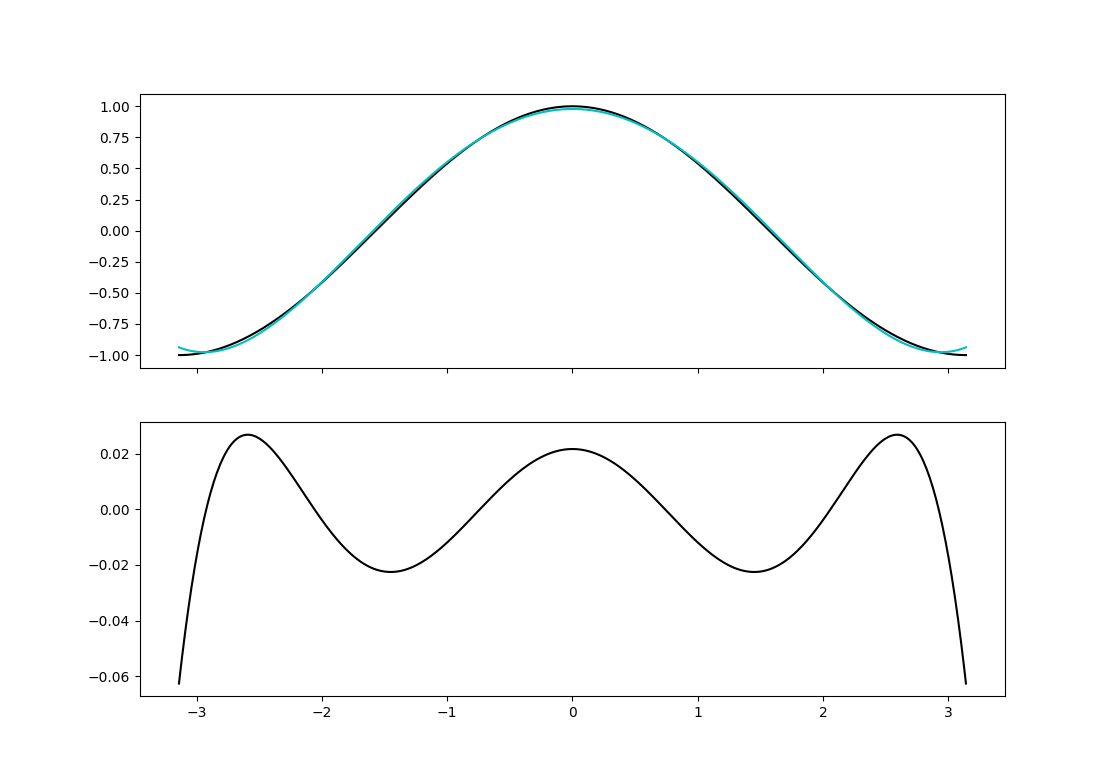
\includegraphics[width=1.0\textwidth]{hw6_p4_fig1}
		\label{legendre_approx}
		\centering
	\end{figure}

	The error is the largest near the ends of the domain. 
	
%%%%%%%%%%%%%%%%%%%%%%%%%%%%%%%%%%%%%%%%%%%%%%%%%%%%%%%%%%%%%%%%%%%%%%%%%%%%%%%%%%%%%%%%%%%%%%%%%%%%
\problem{5 (a)} See the attached Maple printout. It verifies that the first 4 terms are accurate. \\
\cleardoublepage

%%%%%%%%%%%%%%%%%%%%%%%%%%%%%%%%%%%%%%%%%%%%%%%%%%%%%%%%%%%%%%%%%%%%%%%%%%%%%%%%%%%%%%%%%%%%%%%%%%%%
\problem{5 (b)} 

	\begin{figure}[h]
		\caption{The errors of the Taylor Series (red) and Chebyshev Series (blue) approximations to $arctan$.}
		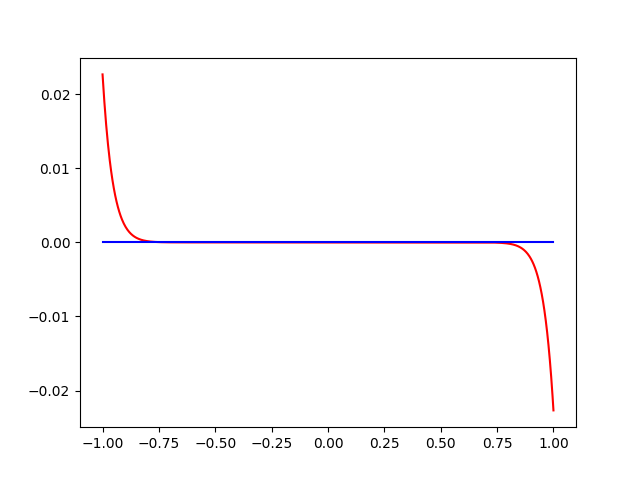
\includegraphics[width=1.0\textwidth]{hw6_p5_fig1}
		\label{arctan_approx}
		\centering
	\end{figure}
	
	As predicted the Chebyshev Series is a much better approximator over a larger interval.
	
	\begin{lstlisting}
def taylor_series(x):
	sum = 0
	for i in range(11):
		sum += (-1)**i /(2*i+1) * x**(2*i+1)
	return sum
def cheb_series(x):
	sum = 0
	alpha = np.sqrt(2)-1
	coef = np.zeros(11*2+1)
	for i in range(11):
		coef[2*i+1] = 1
		sum += (-1)**i /(2*i+1) * alpha**(2*i+1) * 
Chebyshev(coef)(x)
		coef[2*i+1] = 0
	return 2*sum

def p5b():
	x = np.linspace(-1, 1, 1000)
	y = np.arctan(x)
	yt = taylor_series(x)
	yc = cheb_series(x)
	plt.plot(x, y-yt, 'r-')
	plt.plot(x, y-yc, 'b-')
	plt.show()
	print('Max error for Taylor Series: ', np.max(y-yt))
	print('Max error for Chebyshev Series: ', np.max(y-yc))
	
Output: 
Max error for Taylor Series:  0.022680788954
Max error for Chebyshev Series:  1.61917090846e-10
	\end{lstlisting}


		
\end{document}
